\subsection{Orca}
\label{subsec:spec:Orca}
Orca~---~метод поиска аномалий без учителя, использующий подход «ближайшего соседа» (nearest neighbor) для поиска аномалий~\cite{SchwabacherMachLearnAppl}. Данный метод был разработан Стефеном Бэйем (Institute for the Study of Learning and Expertise) и Марком Швабахером (NASA Ames Research Center) и подробно описан в~\cite{BaySchwabacherOrca}. Orca относится к методам обнаружения аномалий, основанных на измерении расстояний между точками (distance-based).

Понятие аномалии для данного класса методов определено следующим образом: «объект $O$ в выборке $T$ является аномалией, если по крайней мере доля $p$ из всех объектов в $T$ лежит дальше от $O$, чем расстояние $D$»~\cite{KnorrNgDistBasedAlgorithms}. Distance-based методы являются обобщением некоторых статистических тестов на аномальность. Данный класс методов не требует априорных знаний о виде распределения для выборки. Кнорр и Нг предложили простейший алгоритм на вложенных циклах (Nested Loop, NL)~\cite{KnorrNgDistBasedAlgorithms}, который находит аномалии путём вычисления расстояния между всеми точками в исходной выборке. Сложность данного алгоритма составляет $O(kN^2)$, где $k$ --- размерность пространства, а $N$ --- размер выборки.

Несмотря на то, что были разработаны более эффективные c т.з. вычислительной сложности алгоритмы (\cite{TaoMiningDistBasedOutliersFromLargeDB}~и~\cite{AngiulliVeryEfficientMiningDistBasedOutliers}), на практике наиболее сложным является определение расстояния $D$, по достижению которого точку следует считать аномалией. Может потребоваться непредсказуемо большое число итераций, чтобы найти подходящее значение $D$. Найти интервал $[D_{min}, D_{max}]$ возможно путём полного перебора, как показано в~\cite{TaoMiningDistBasedOutliersFromLargeDB}, но данный подход обладает слишком высокой вычислительной сложностью.

В качестве решения данной проблемы было предложено следующее определение аномалии, не требующее задания $D$: «объект считается аномалией, если это один из $n$ объектов с наибольшим расстоянием до их $k$-ых ближайших соседей, где~\mbox{$k,n\in\mathbb{N}$}»~\cite{RamaswamyEffAlgoMiningOutliers}. Пример показан на рисунке\ref{fig:spec:Orca:NearestNeighbor}. Пользователю достаточно указать количество аномалий, которое должен вернуть алгоритм, без прямого указания дистанции $D$. Более того, возвращаемые алгоритмом аномалии будут ранжированы по степени аномальности, являющейся численной характеристикой.

\begin{figure}
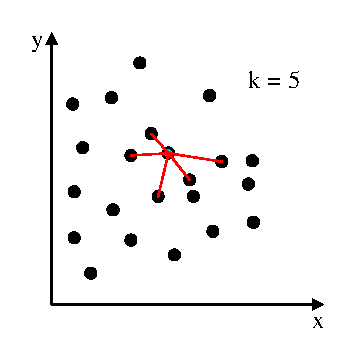
\includegraphics[width=0.5\textwidth]{nearest_neighbors}
\caption{Ближайшие соседи точки для двухмерного случая при $k=5$}
\label{fig:spec:Orca:NearestNeighbor}
\end{figure}

Orca использует данный подход, развивая идею алгоритма на вложенных циклах~(NL). Данный алгоритм на больших массивах данных показывает сложность, близкую к линейной~\cite{BaySchwabacherOrca}. Псевдокод алгоритма приведён в листинге~\ref{lst:spec:OrcaPseudocode}. Блок-схема показана на рисунке~\ref{fig:spec:Orca:Scheme}.

\begin{algorithm}[h!]
\caption{Псевдокод алгоритма Orca}
\label{lst:spec:OrcaPseudocode}
\begin{algorithmic}[1]
\REQUIRE $k$, количество ближайших соседей; $n$, количество аномалий; $D$, выборка
\ENSURE $O$, множество аномалий
\STATE Перемешать все объекты в выборке $D$. \label{lst:spec:OrcaPseudocode:Random}
\STATE Инициализировать величину среза нулём
\WHILE{в выборке $D$ остались необработанные объекты}
	\STATE Загрузить фиксированное количество объектов $B$ в буфер
	\FOR{каждого объекта $d$ в $D$} \label{lst:spec:OrcaPseudocode:NL}
		\FOR{каждого объекта $b$ в $B$}
			\STATE Вычислить расстояние между $b$ и $d$.
			\IF{$d$ ближе к $b$, чем $k$ ближайших соседей $b$}
				\STATE Заменить соседа с наибольшим расстоянием на $d$
				\STATE Вычислить степень аномальности $b$
				\IF{степень аномальности ниже величины среза} \label{lst:spec:OrcaPseudocode:Pruning}
					\STATE Удалить $b$ из $B$
				\ENDIF
			\ENDIF
		\ENDFOR
	\ENDFOR
	\STATE Поместить в $O$ оставшиеся в $B$ объекты
	\STATE Отсортировать объекты в $O$ по степени аномальности
	\STATE Оставить в $O$ только $n$ объектов
	\STATE Обновить величину среза степенью аномальности последнего объекта в $O$
\ENDWHILE
\RETURN $O$
\end{algorithmic}
\end{algorithm}

\begin{figure}
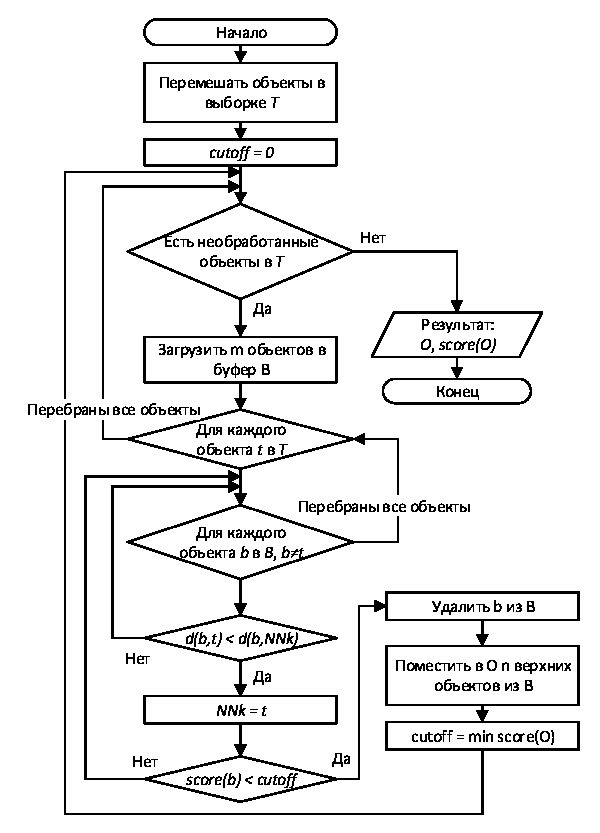
\includegraphics[height=0.5\textheight]{orca_scheme}
\caption{Блок-схема алгоритма Orca}
\label{fig:spec:Orca:Scheme}
\end{figure}

Ключевыми особенностями алгоритма являются:
\begin{itemize}
	\item необходимость рандомизации исходных данных (строка~\ref{lst:spec:OrcaPseudocode:Random}). Для эффективной работы алгоритма требуется, чтобы объекты в выборке находились в случайном порядке. При обработке выборки на ПЗУ возможно рандомизировать выборку за линейное время и используя конечный объём памяти~\cite{BaySchwabacherOrca};
	\item использование вложенных циклов (строка~\ref{lst:spec:OrcaPseudocode:NL}). Основной идеей является отслеживание ближайших соседей для каждого объекта в $D$;
	\item правило отсечения (строка~\ref{lst:spec:OrcaPseudocode:Pruning}). Когда для ближайших соседей объекта степень аномальности становится меньше, чем величина среза, алгоритм удаляет данный объект, так как больше нет оснований считать его аномальным. Чем больше объектов перебирает алгоритм, тем выше становится величина среза, улучшая таким образом эффективность алгоритма по времени.
\end{itemize}

В качестве метрики для определения расстояния может использоваться, к примеру, Евклидово расстояние для непрерывных и расстояние Хэмминга для дискретных переменных. Функция, определяющая степень аномальности, может быть любой монотонно убывающей функцией от расстояний до ближайших соседей~\cite{BaySchwabacherOrca}, например, среднее расстояние до $k$ ближайших соседей или расстояние до $k$-го ближайшего соседа.

Преимуществами метода являются:
\begin{itemize}
	\item превосходная масштабируемость: на выборках большого объёма производительность алгоритма близка к линейной;
	\item низкие требования к памяти: не требуется загружать в память всю выборку;
	\item возможность задать любую метрику для расстояния и функцию для определения степени аномальности.
\end{itemize}

Недостатки следуют из природы метода. В качестве основных можно выделить следующие:
\begin{itemize}
	\item в худшем случае (например, когда выборка не содержит аномалий) производительность алгоритма крайне низкая. Из-за вложенных циклов может потребоваться $O(N^2)$ операций вычисления расстояния и $O(N/l \cdot N)$ операций доступа к данным, где $l$ --- размер буфера;
	\item в качестве результата алгоритм возвращает фиксированное число аномалий, указанное перед началом работы;
	\item данный метод не способен определять аномальность объекта в реальном времени, так как для этого требуется вычислить расстояние до всех объектов в выборке.
\end{itemize}